\documentclass[conference]{IEEEtran}

\IEEEoverridecommandlockouts

\usepackage{cite}
\usepackage{hyperref}
\usepackage{amsmath,amssymb,amsfonts}
\usepackage{algorithmic}
\usepackage{graphicx}
\usepackage{textcomp}
\usepackage{xcolor}
\usepackage{url}

\def\BibTeX{{\rm B\kern-.05em{\sc i\kern-.025em b}\kern-.08em
    T\kern-.1667em\lower.7ex\hbox{E}\kern-.125emX}}

\begin{document}

\title{A Comparison of Algorithms Playing EvoMan}

\author{\IEEEauthorblockN{Cojocaru Gabriel-Codrin, Dinu Sergiu-Andrei}
\IEEEauthorblockA{\textit{"Alexandru Ioan Cuza" University (UAIC) Iasi} \\
\textit{Faculty of Computer Science}\\
\textit{Computational Optimization Master}\\
Iasi, Romania \\
\{gabriel.cojocaru, sergiu.dinu\}@info.uaic.ro\\
\{gcodrincojocaru, dinusergiuandrei997\}@gmail.com}
\and
}

\maketitle

\begin{abstract}
This paper describes a comparison between algorithms for
evolving agents for the game Evoman.
The algorithms we have tested are Q-learning with neural networks, sparse reward neuroevolution and
iterative neuroevolution algorithms.
Both neuroevolution algorithms were tested with genetic algorithms and particle swarm optimization.
As of the results, the Q-learning approach lead to the worst results.
There was no significant difference between the performance of the iterative neuroevolution
and the sparse neuroevolution when used with genetic algorithms.
When particle swarm optimization was used, the iterative approach lead to worse results than the sparse one.
Both of the neuroevolutions with particle swarm optimization lead to much better results than both of the
neuroevolutions with genetic algorithms.
We have also shown that there is not a significant change in the performance of sparse neuroevolutive
algorithms with particle swarm optimization even when the cognitive and social weights suffer great changes.
\end{abstract}

\begin{IEEEkeywords}
game-playing agent, artificial intelligence, EvoMan, genetic algorithm, reinforcement learning,
q-learning, neuroevolution, particle swarm optimization
\end{IEEEkeywords}

\section{Introduction}\label{sec:introduction}
EvoMan~\cite{karinemiras,evoman} is a framework for testing competitive game-playing agents.
This framework is inspired by Mega Man II~\cite{capcom}, the game created by Capcom.
In the original game, the player would have to beat $8$ opponents and acquire their weapons
as they are defeated.
The additional difficulty of EvoMan comes from the fact the player has to defeat all
the opponents using only the starting weapon.
The framework is freely available\footnote{\url{https://github.com/karinemiras/evoman_framework}}
and it is currently compatible with Python 3.6 and 3.7.
There is also an extensive documentation
available\footnote{\url{https://github.com/karinemiras/evoman_framework/blob/master/evoman1.0-doc.pdf}}.

The agent will collect information about the environment through 20 sensors (Fig 1):
\begin{itemize}
    \item 16 correspond to horizontal and vertical distances to a maximum of 8 different opponent projectiles.
    \item 2 correspond to the horizontal and vertical distance to the enemy.
    \item 2 describe the directions the player and the enemy is facing
\end{itemize}
\begin{figure}
    \centering
    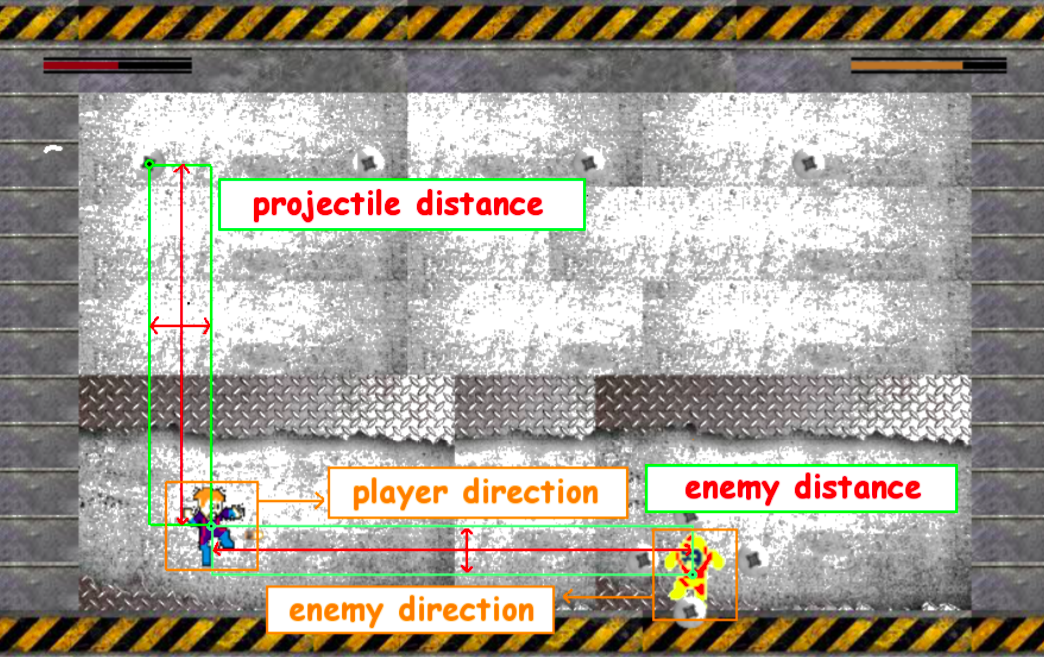
\includegraphics[width=0.5\textwidth]{images/Evoman3.png}
    \caption{Sensors available for the player.}
    \label{fig:sensors}
\end{figure}
The actions which the agent may take are:
\begin{itemize}
    \item walk left
    \item walk right
    \item jump
    \item shoot
    \item release of the jump
\end{itemize}

The lives of the player and the enemy start at 100.
Everytime one of them gets hit, their life deplenishes.
Whoever's life reaches 0 loses the game.

In our work, we have focused on the designing specialized models able of learning how to win a
match against specific enemies of each level.

\section{Method}\label{sec:method}
The formula used for evaluating an agent is:

\boldmath
\begin{gather*}
    0.9 * (100 - enemy\_life) + 0.1 * player\_life\\
    - ln(nr\_of\_game\_timesteps)\\
\end{gather*}
\unboldmath
We have decided to reduce the fitness in time in order to encourage the agents to be active.
We are mainly rewarding the damage done to the opponent, while also considering, but with less importance,
the player's life.
\newpage
The author defines a success criterion for a solution as:
\begin{itemize}
    \item Effectiveness: to zero the life of the enemy.
    \item Efficiency: the amount of life preserved by the player.
\end{itemize}
From our reward function, it is visible that we have biased our models towards effectiveness,
rather than efficiency.
This decision is solely based on intuition.

We have tested five algorithms to control the EvoMan agent.

\subsection{Q-learning with Neural Networks}\label{subsec:q-learning-with-neural-network}
The first algorithm is a classic Q-learning\cite{q_learning} algorithm with neural networks which we have used
as a baseline model.

We used a neural network to predict the reward function for each possible move
(left, right, shoot, jump, release of jump) from a given state.
We then take the action with the highest predicted reward.
The input of this neural network is composed of the current game sensors and the
previous 2 game sensors with the moves taken at that specific point.

The neural network used for experiments has 2 hidden layers with 32 neurons each.
Each layer has l2 regularization applied with a weight decay of 0.01 and sigmoid activation.
After each predicted move, we updated the neural network using backpropagation,
using as input the game sensors and as output the true reward function.
We have trained the agent on 5000 games.

\subsection{Sparse Reward Neuroevolution}\label{subsec:sparse-reward-neuroevolution}
The second algorithm is a sparse reward neuroevolution\cite{neuro}.
We called it "sparse" reward because an agent doesn't find out how well it's doing until
the end of the game, with no feedback during the game.
An individual is represented as the weights of a neural network.

The neural network role is to predict the next move using the current game sensors and
the previous 2 game sensors with the moves taken at that specific point.
We used 2 hidden layers with 32 neurons for each individual.

We start with randomly initialized neural network weights and then represent them as a bitstring.
The weights used for the neural network were values between 2 and -2 with a precision of 6 digits.

The search of individuals that lead to good fitness values can not be done with evolutive algorithms.

For evaluation, the bitstring is transformed into the weights of the neural network and a game is played,
from which we can obtain the individual fitness.

\begin{itemize}
    \item Genetic Algorithms\cite{genetic_algorithm} \\
    Since we are already representing our individuals as bitstrings, the classical operations of a
genetic algorithm on bits can be applied: crossover, mutation and selection.
    The configurations used for the genetic algorithm are:
    \begin{itemize}
        \item population size 50
        \item number of generation 500
        \item crossover rate 0.7
        \item mutation rate 0.008 and 0.1
    \end{itemize}
    The solution of the genetic algorithm is the best individual from the last generation.
    \newpage
    \item Particle Swarm Optimization\cite{pso} \\
    The configurations used for the particle swarm optimization algorithm are:
    \begin{itemize}
        \item population size 30
        \item number of iterations 200
        \item cognitive weight 0.4 - 0.8 - 1.5
        \item social weight 0.8 - 0.4 - 3
    \end{itemize}
\end{itemize}

\subsection{Iterative Neuroevolution}\label{subsec:iterative-neuroevolution}
The last algorithm is an iterative neuroevolution.
We called it "iterative" because the agents are trained on a small number of game steps
first and then the number of game timesteps slowly increases.

After a number generations we increase the number of game timesteps the agents are allowed to train on.
The fitness function was scaled based on the number of game timesteps in a way that if an agent
training on x game timesteps will always have a fitness lower than an agent training on y game
timesteps if x is lower than y.

We used the same genetic algorithm, neural network configuration and
very similar particle swarm optimization configurations as the ones for the sparse reward neuroevolution.
The difference in configuration of the neuroevolution with particle swarm optimization is that we are
no longer testing configurations using only a constant inertia weight.
The new try is with a uniformly decreasing inertia weight with respect to the percent of the iterations passed,
having values from 1 to 0.3.

\section{Experiment}\label{sec:experiment}
For the highest game difficulty, for all algorithms we have run 30 experiments.
For both neuroevolutive algorithms we used the same size for the neural network of an
individual while the reward predictor neural network used in Q-learning had the same size.
We also tried to balance the number of iterations used for training the genetic algorithms
and particle swarm optimization algorithms with the number of games the Q-learning agent trains on. \\

Especially in the case of the neuroevolution with particle swarm optimization, the algorithm configurations were
tested and decided empirically along the way. \\

When decreasing the game difficulty to observe how the best model behaves in increasingly easier environments,
the number of experiments was not fixed and was determined by a fixed time frame equal to 16 hours.
This lead to a number of runs per difficulty level varying from 10 to 24.
This liberty was taken due to the fact that the results of such an experiment are of a lesser importance than the ones
at the highest difficulty.

\newpage
\section{Results}\label{sec:results}

\begin{figure}[!h]
    \centering
    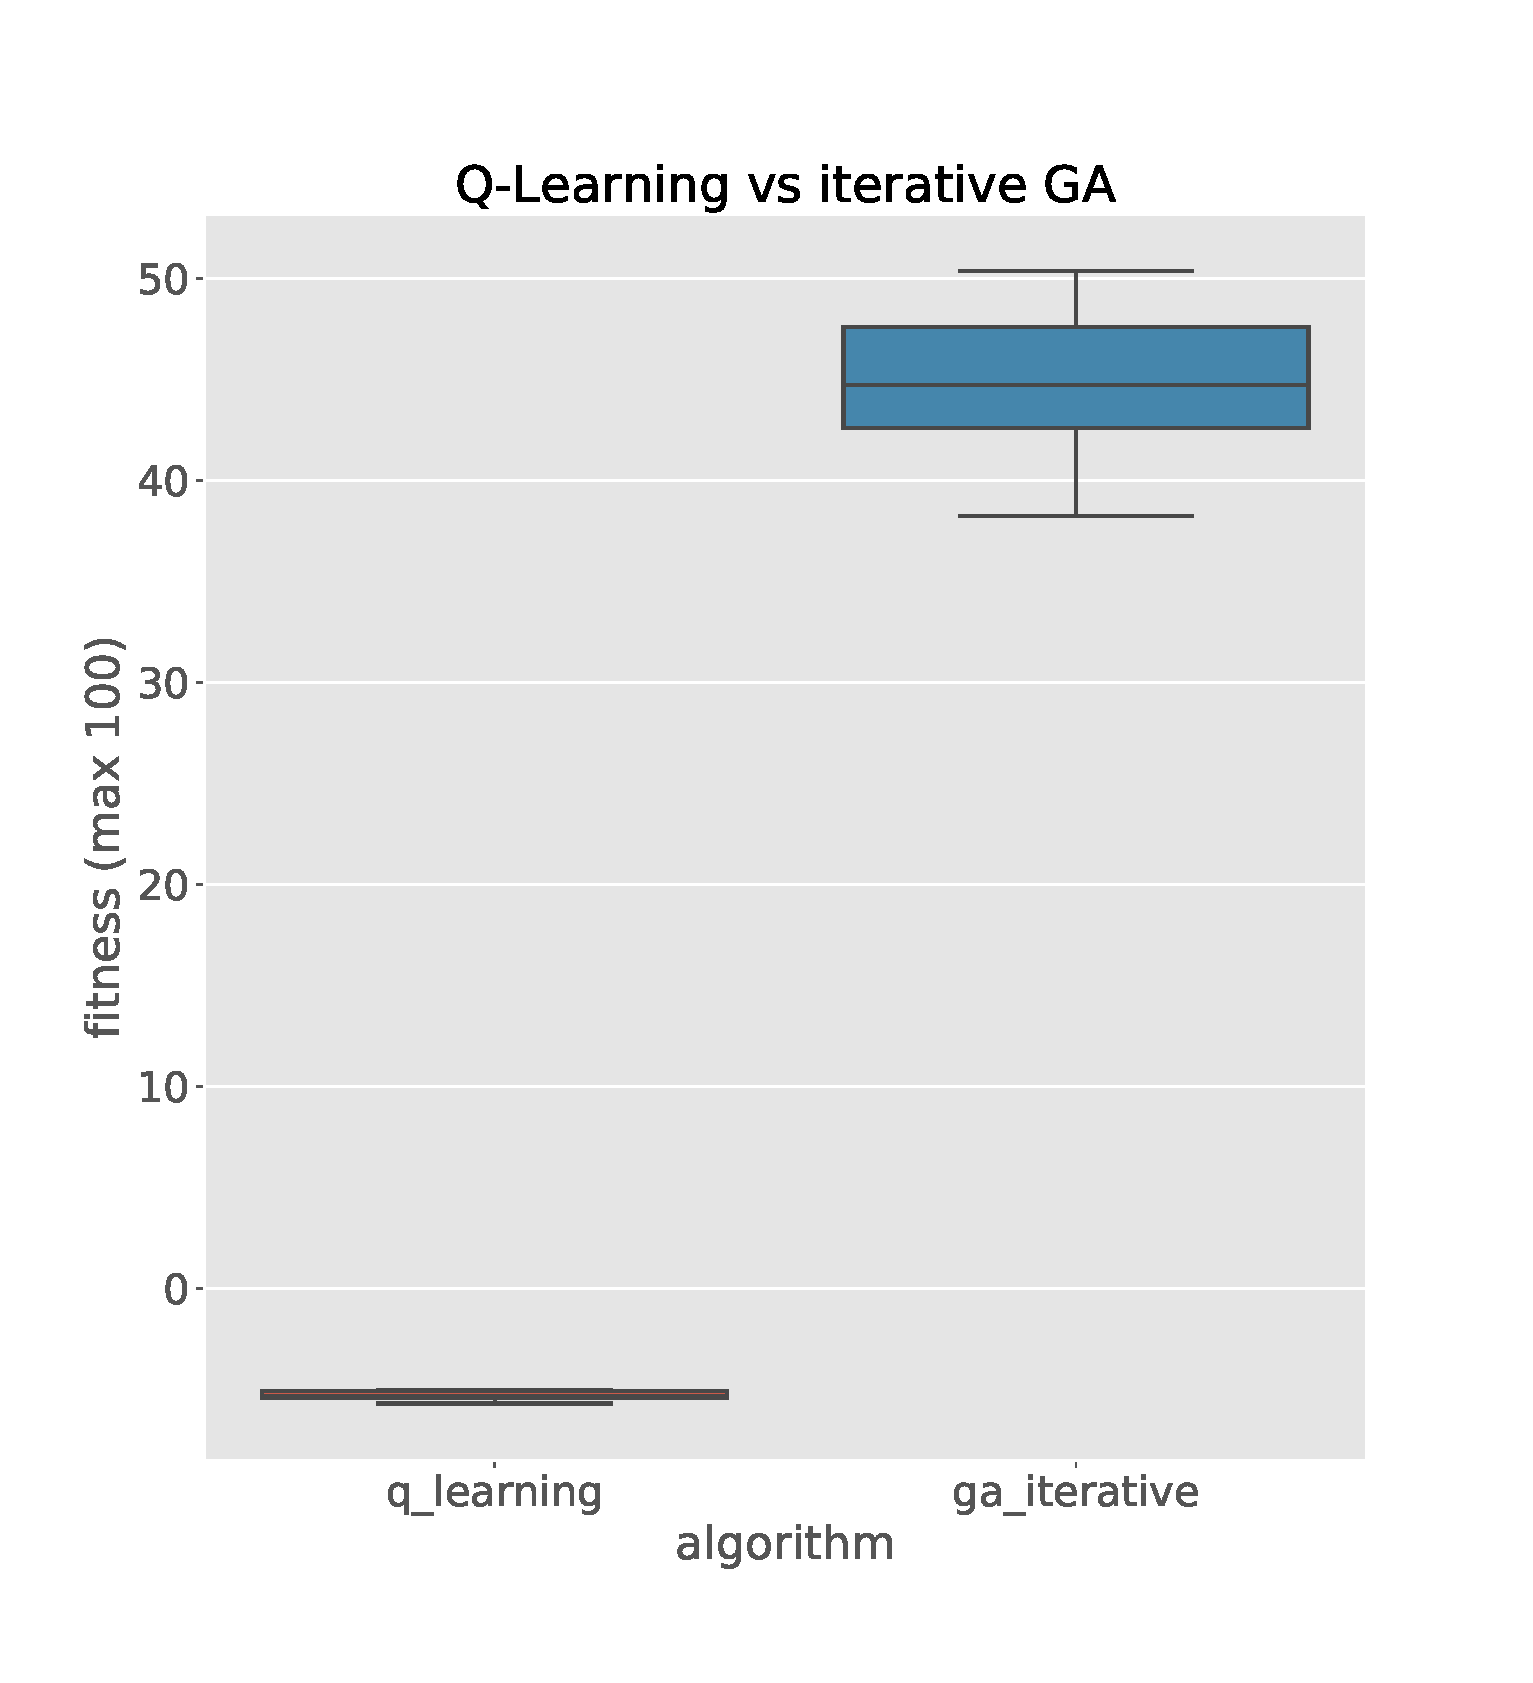
\includegraphics[width=0.5\textwidth]{images/q_vs_ga_iterative.eps}
    \caption{The fitness comparison between Q-learning and iterative neuroevolution with genetic algorithms.}
    \label{fig:q_vs_ga_iterative}
\end{figure}

\begin{figure}[!h]
    \centering
    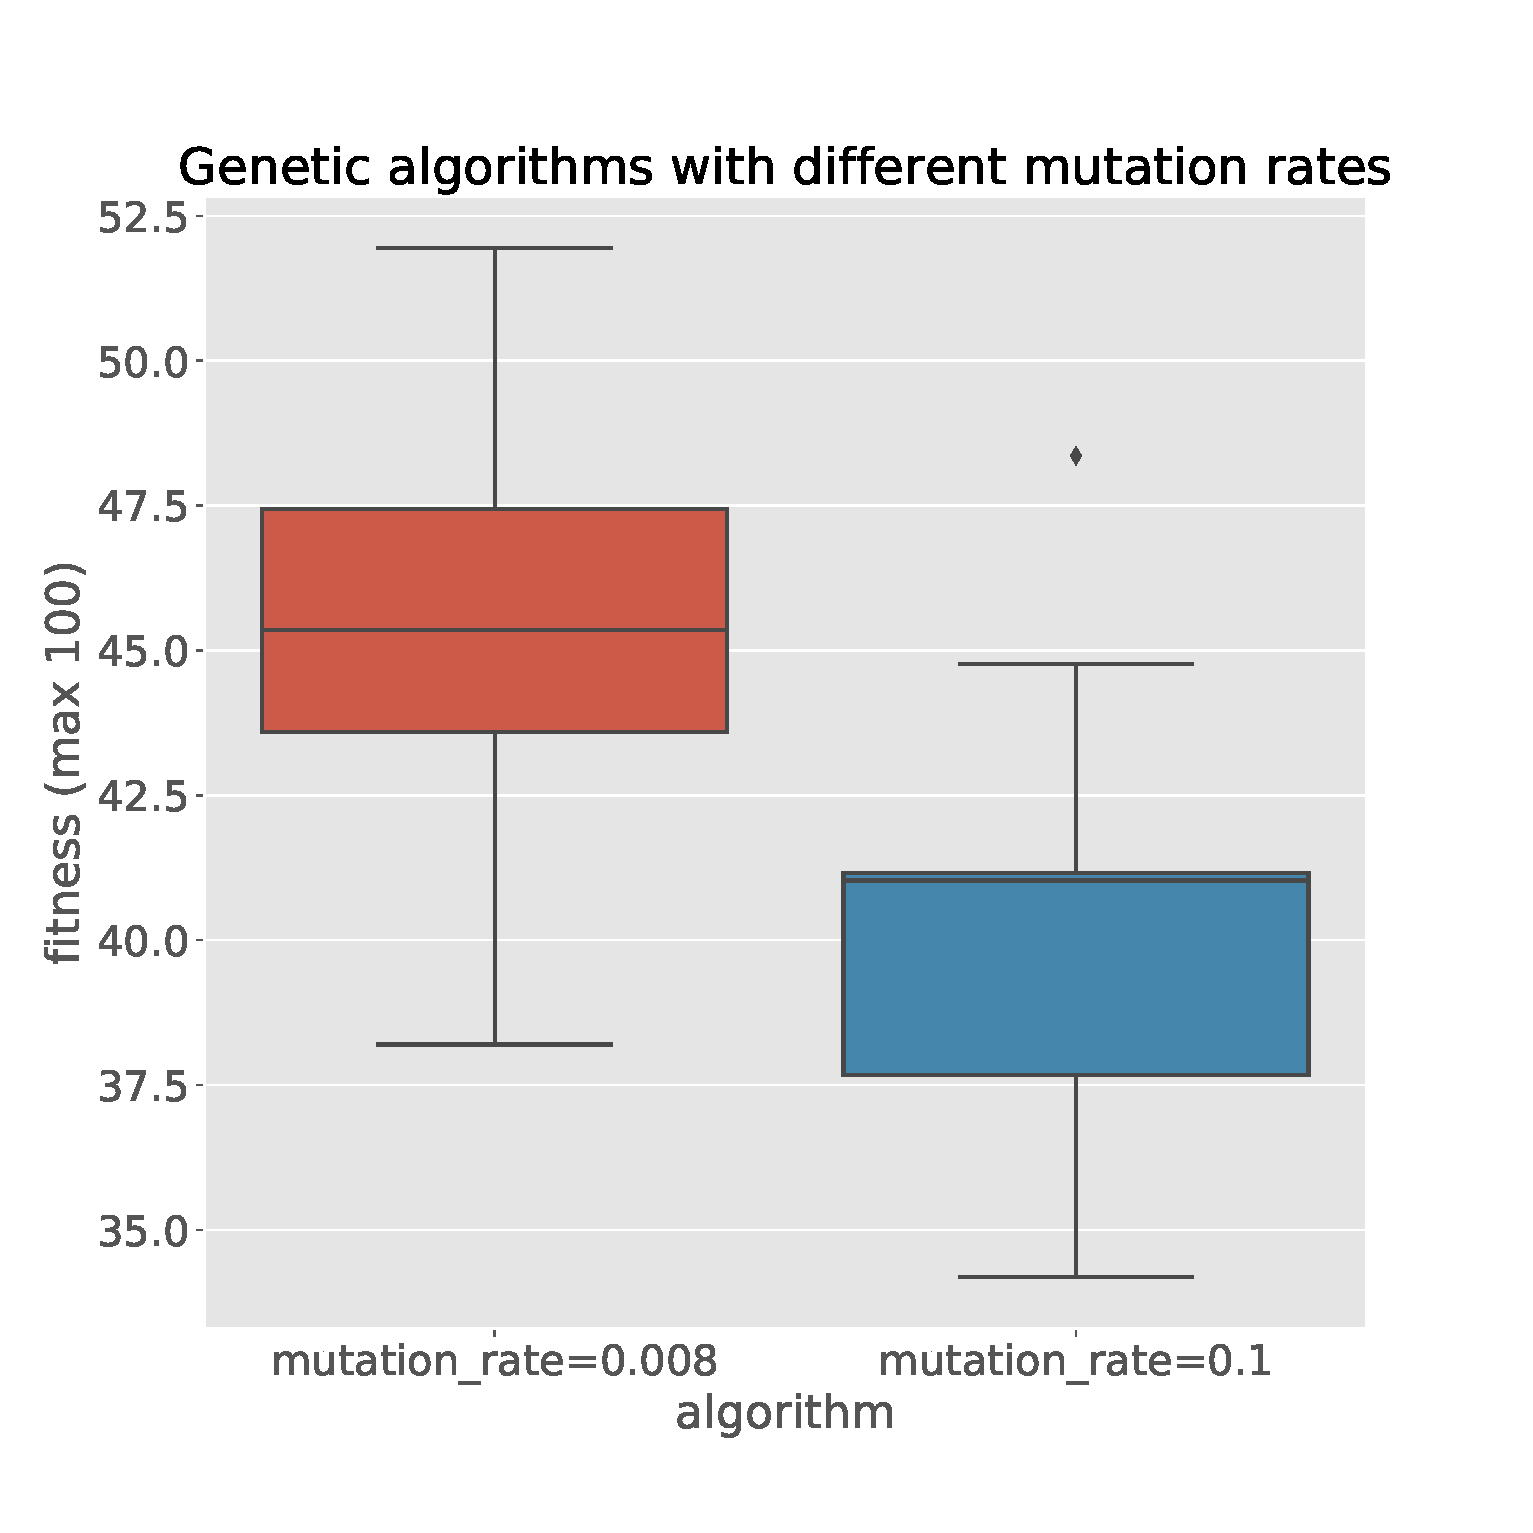
\includegraphics[width=0.5\textwidth]{images/ga_mutation_rates.eps}
    \caption{The fitness comparison between sparse neuroevolutions with genetic algorithms with mutation rate of 0.1 and 0.008.}
    \label{fig:ga_mutation_rates}
\end{figure}

\begin{figure}[!h]
    \centering
    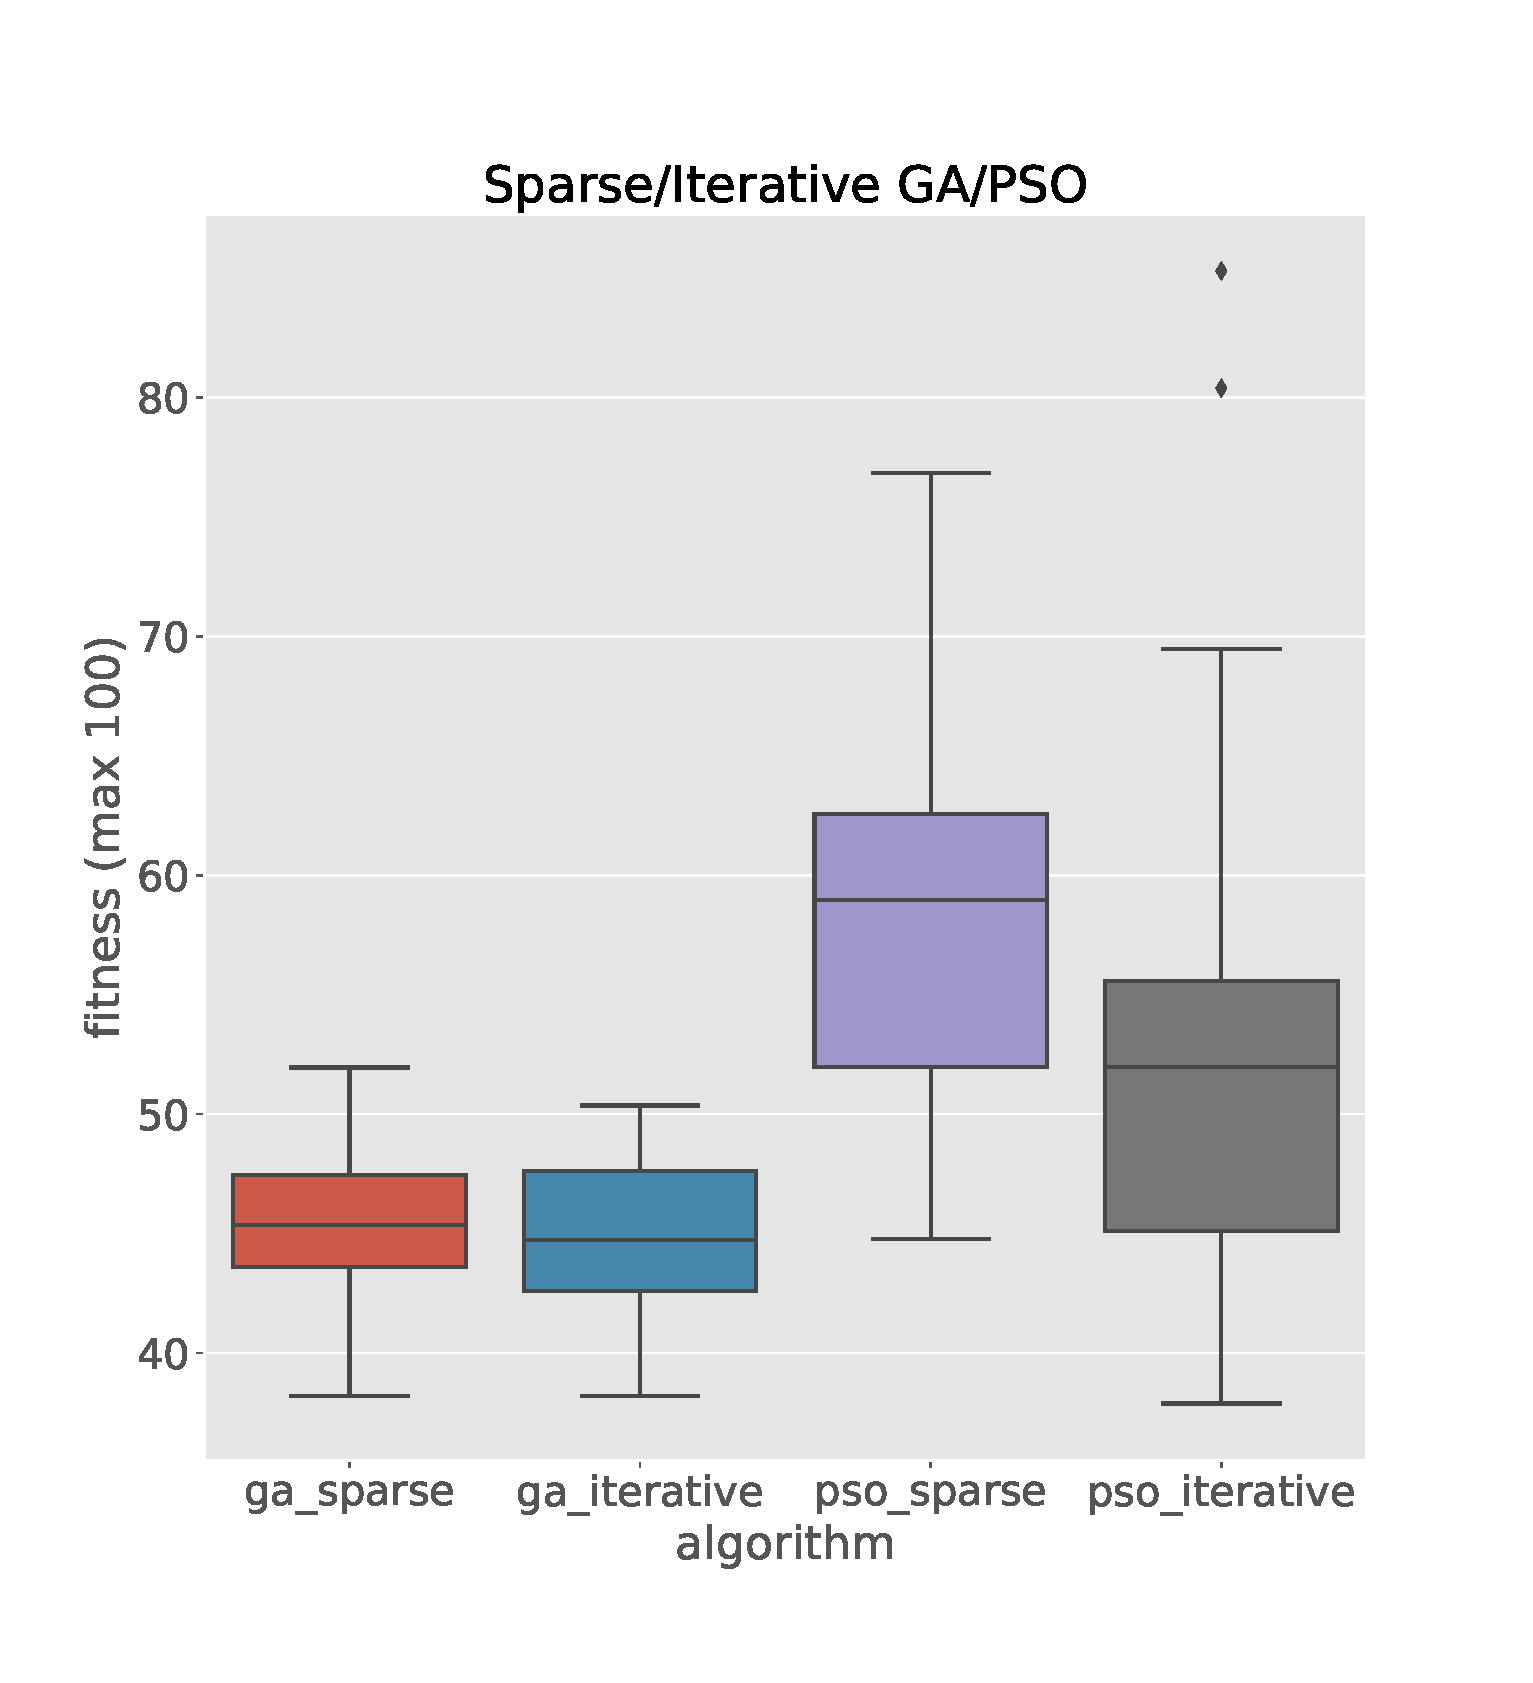
\includegraphics[width=0.5\textwidth]{images/overview.eps}
    \caption{The fitness comparison between the iterative neuroevolution and the sparse neuroevolution,
    both with genetic algorithms and particle swarm optimization algorithms. }
    \label{fig:overview}
\end{figure}

\begin{figure}[!h]
    \centering
    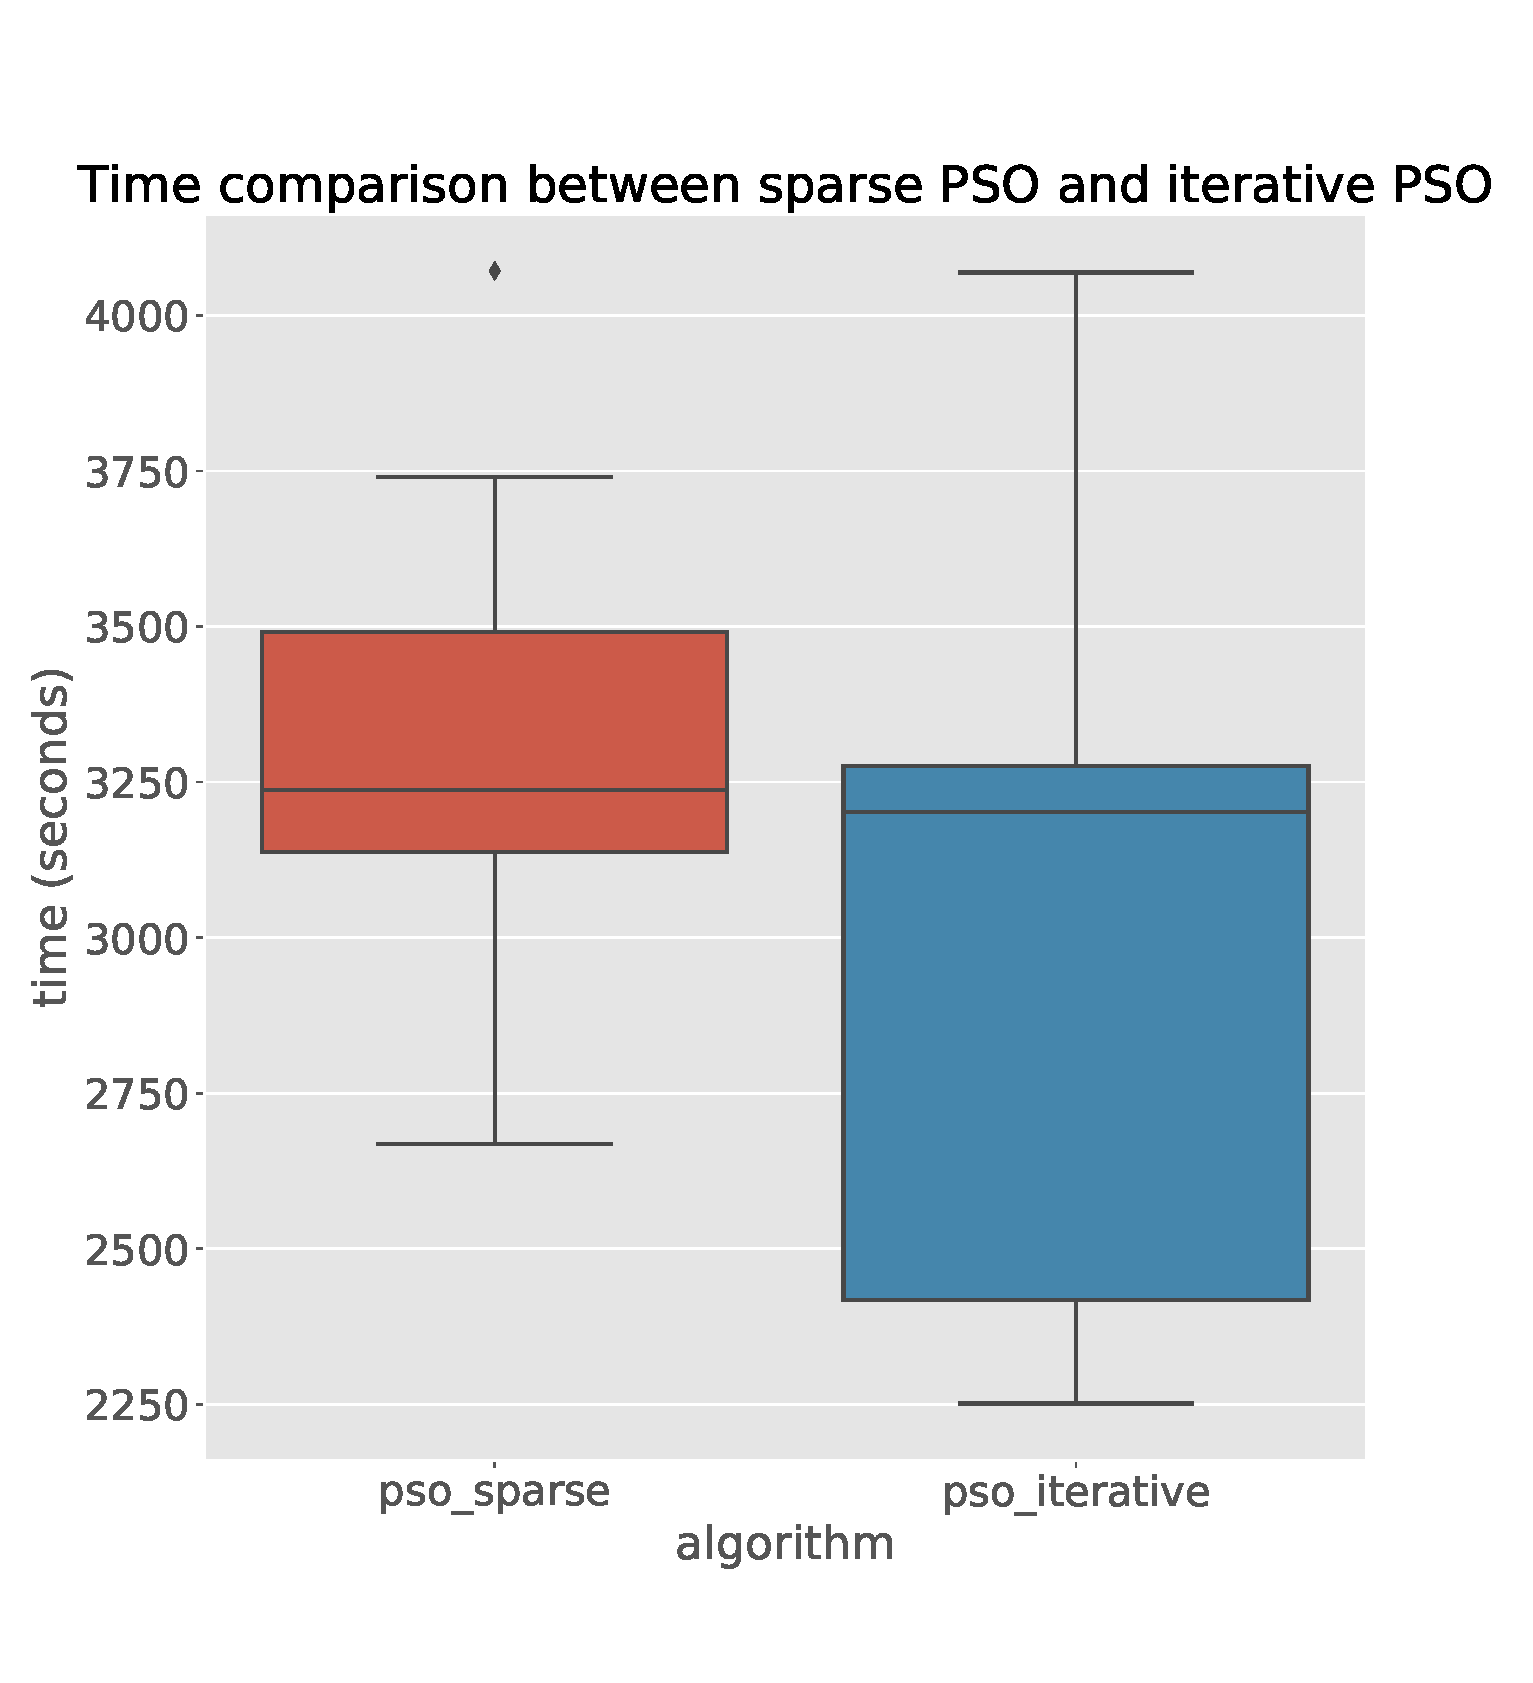
\includegraphics[width=0.5\textwidth]{images/pso_sparse_vs_iterative_time.eps}
    \caption{The time comparison between sparse and iterative neuroevolutions with particle swarm optimization.}
    \label{fig:pso_sparse_vs_iterative_time}
\end{figure}


\begin{figure}[!h]
    \centering
    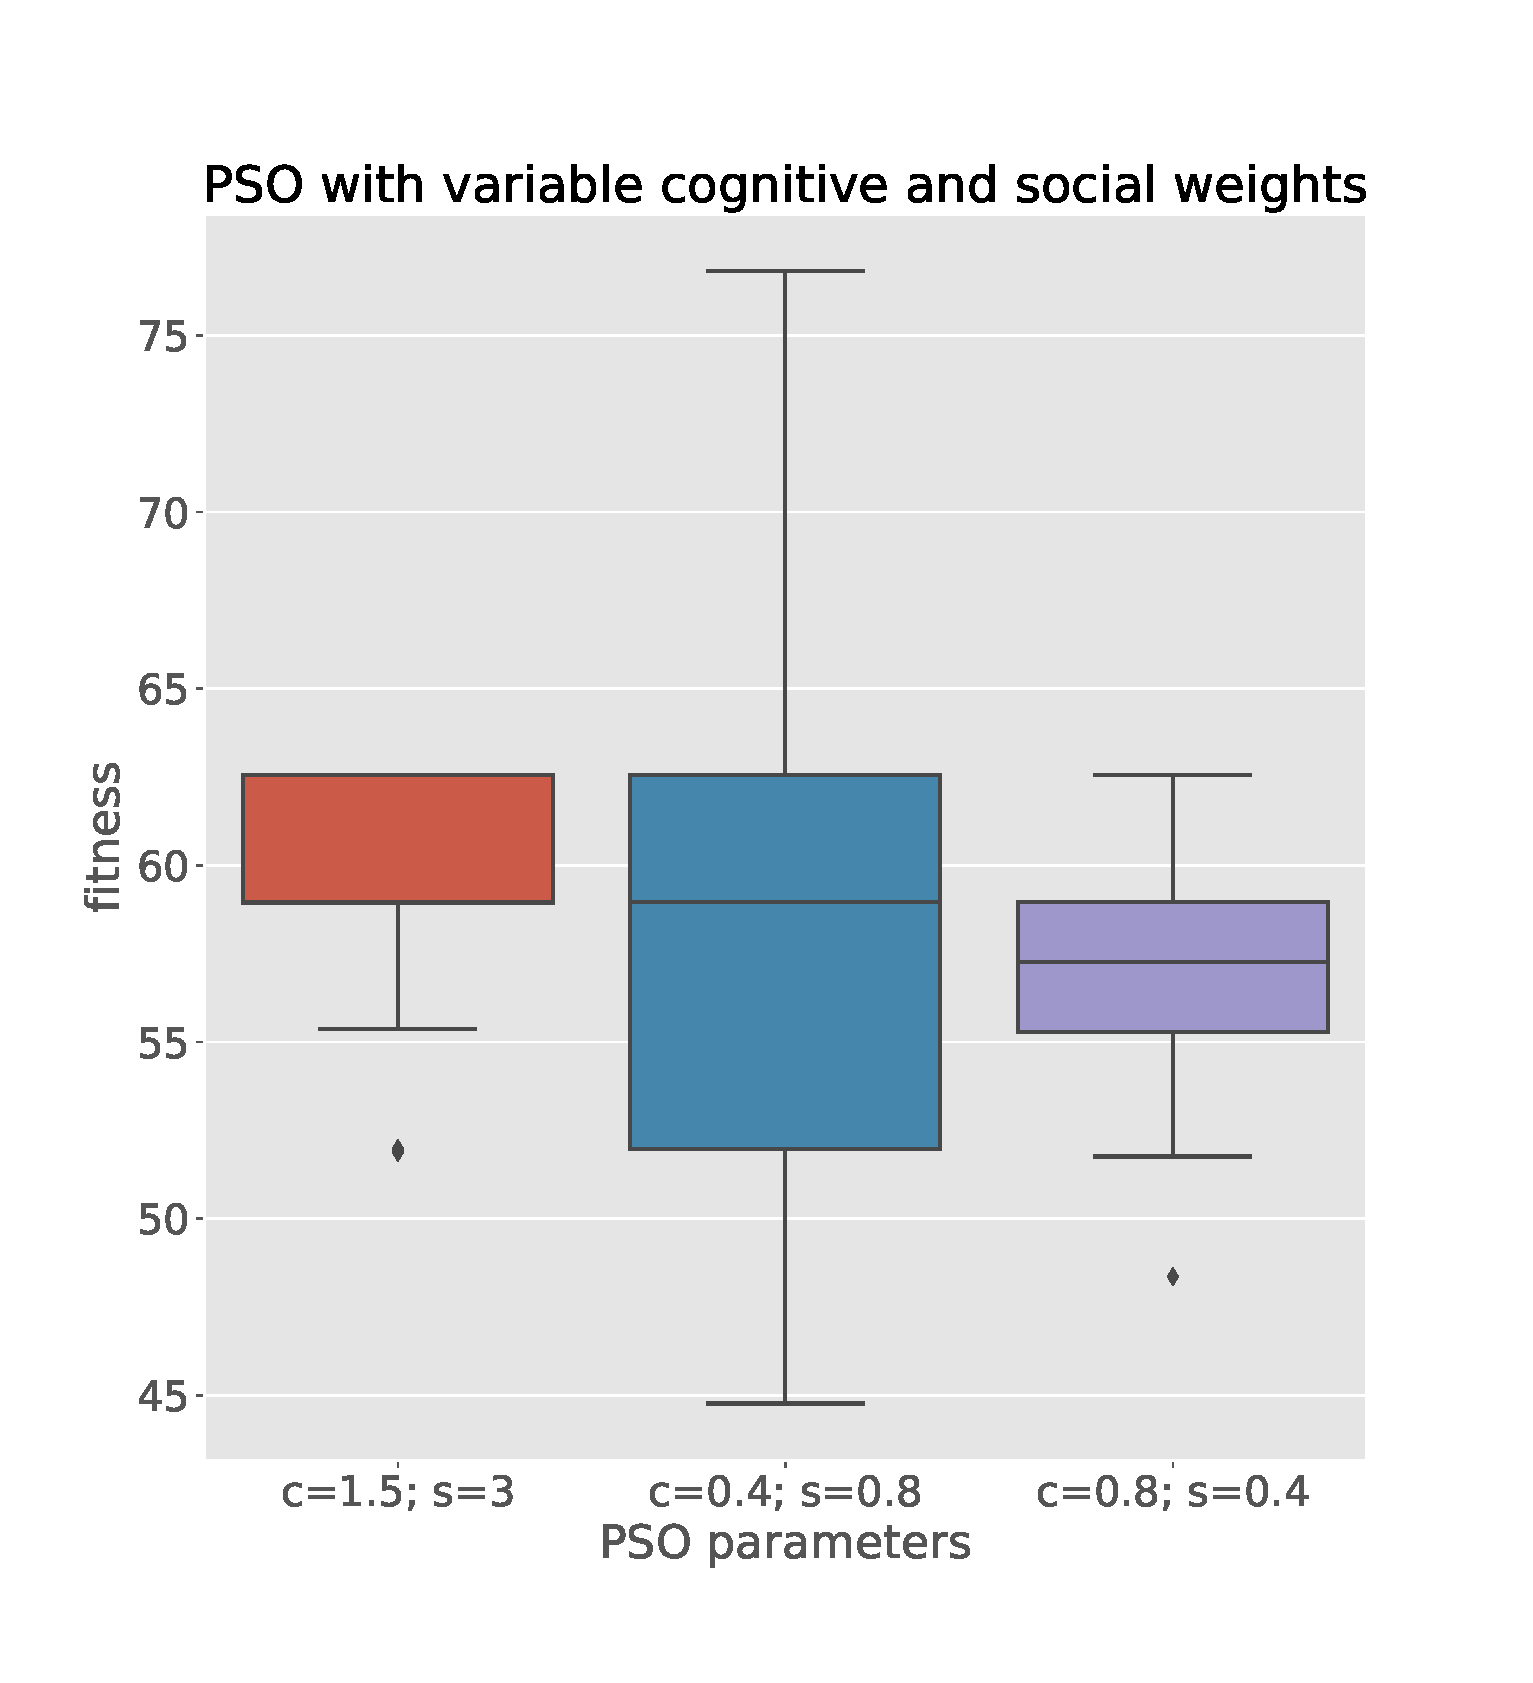
\includegraphics[width=0.5\textwidth]{images/pso_configs.eps}
    \caption{The fitness comparison between sparse neuroevolutions with particle swarm optimization
    with different cognitive and social weights.}
    \label{fig:pso_configs}
\end{figure}


\begin{figure}[!h]
    \centering
    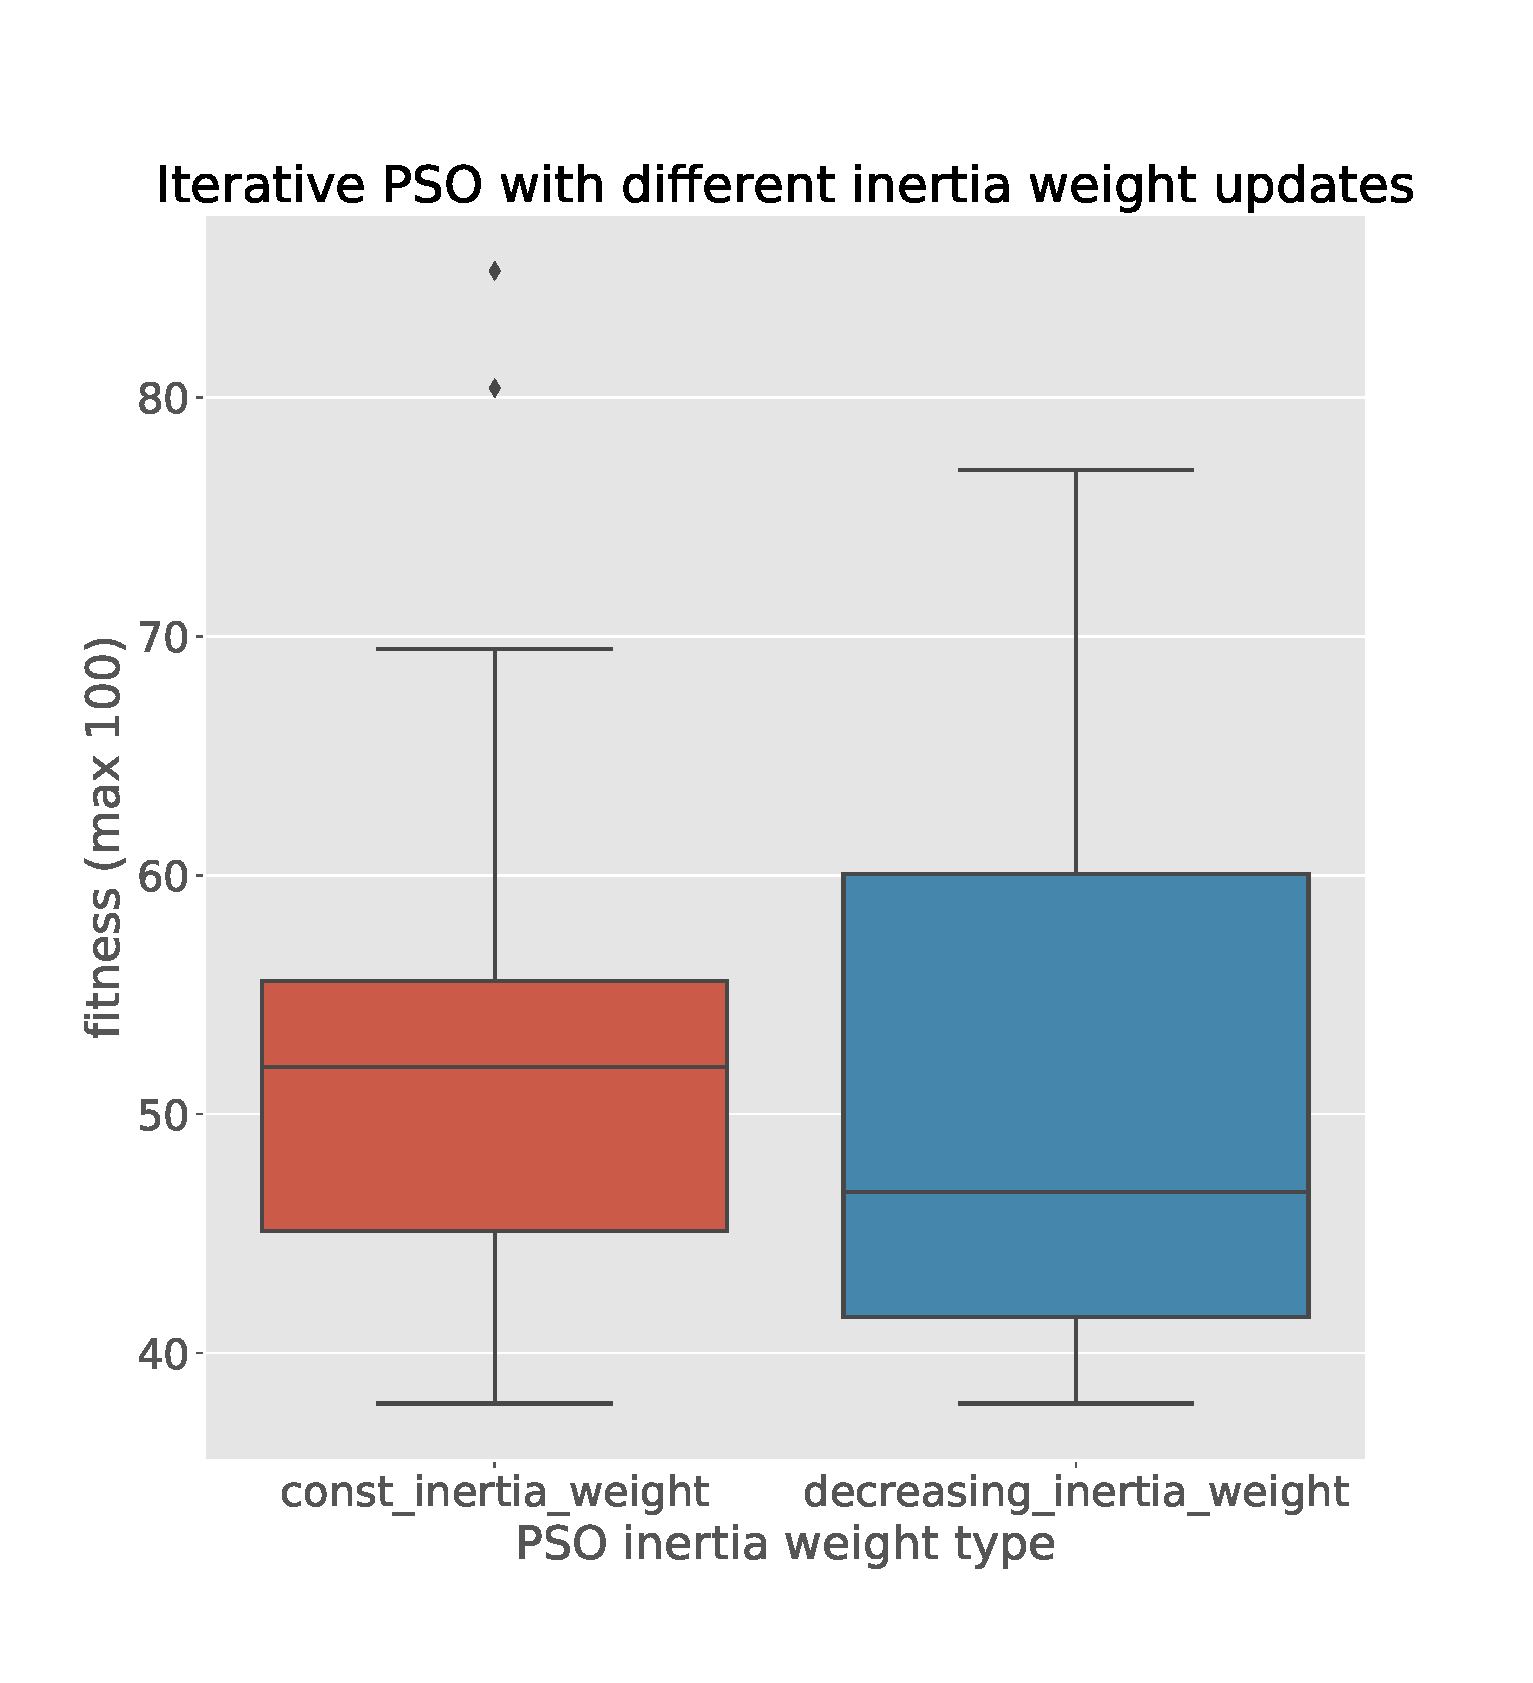
\includegraphics[width=0.5\textwidth]{images/pso_inertia.eps}
    \caption{The fitness comparison between neuroevolutions with particle swarm optimization with constant inertia
    weight and with uniformly decreasing in time inertia weight.}
    \label{fig:pso_inertia}
\end{figure}


\begin{figure}[!h]
    \centering
    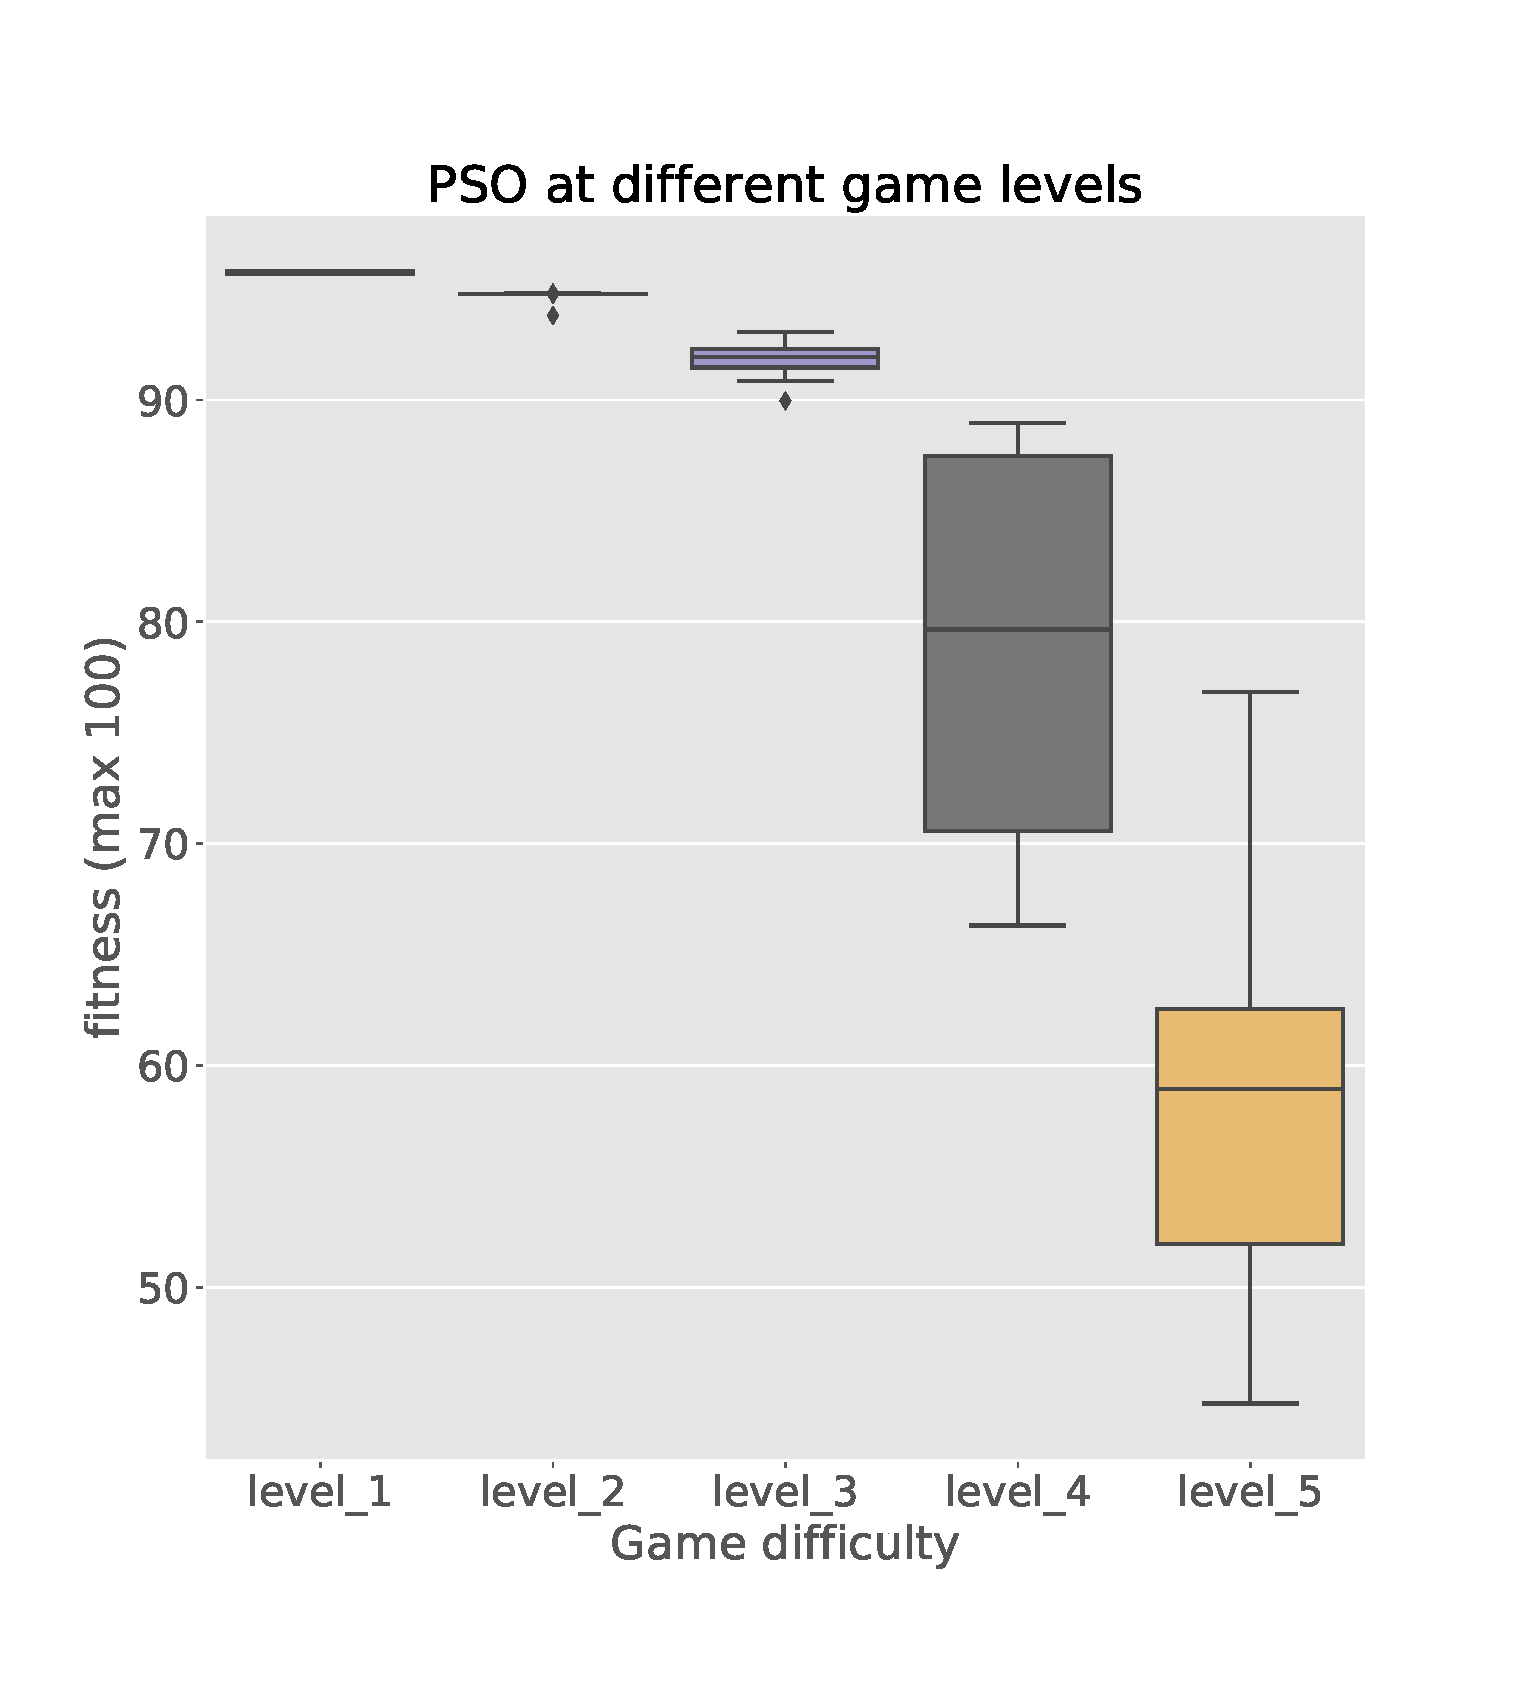
\includegraphics[width=0.5\textwidth]{images/pso_levels.eps}
    \caption{The fitness comparison of neuroevolutions at different game difficulty levels.}
    \label{fig:pso_levels}
\end{figure}


\begin{figure}[!h]
    \centering
    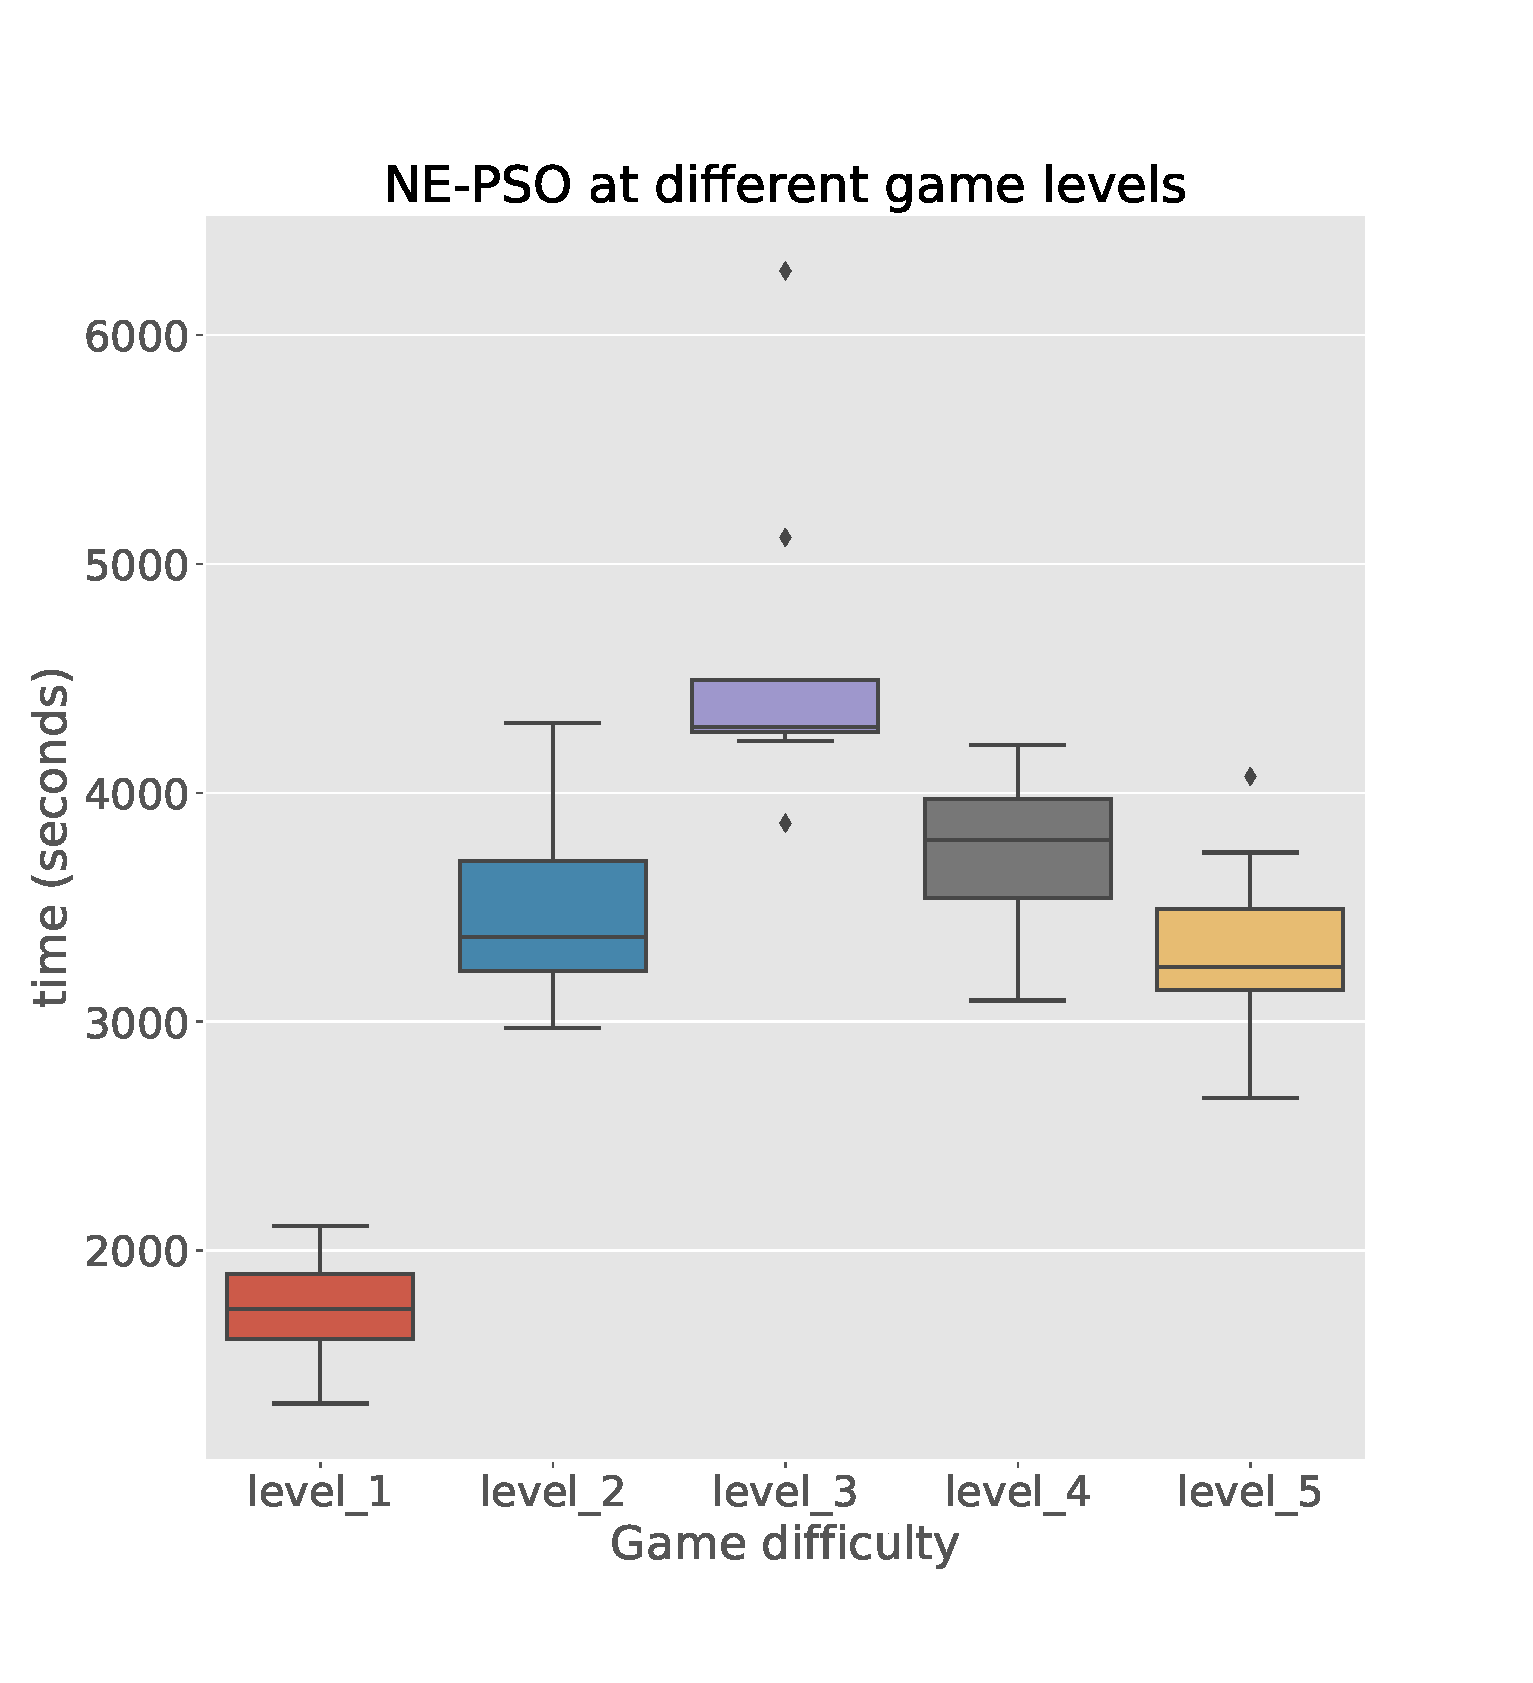
\includegraphics[width=0.5\textwidth]{images/pso_levels_time.eps}
    \caption{The time comparison of neuroevolutions at different game difficulty levels.}
    \label{fig:pso_levels_time}
\end{figure}

\newpage

\section{Interpretation of Results}\label{sec:interpretation-of-results}

From Fig.~\ref{fig:q_vs_ga_iterative} we can clearly see that the neuroevolution with the genetic algorithm
lead to much better results than the Q-learning algorithm with neural networks.
Despite running 5000 games, a number of evaluations comparable to the one of the neuroevolution,
the Q-learning algorithm did not manage to successfully train an agent.
The neuroevolution with genetic algorithms lead to a good fitness score, but the resulting agent was not good enough
to win the game.

In Fig.~\ref{fig:ga_mutation_rates} we can see the fitness comparison between neuroevolutions with genetic algorithms
with extremely different mutation rates.
This was tried with the hope that the high mutation rate could lead to a better exploration of the game space.
This problem lead to the usual intuition of a genetic algorithm stating that a high mutation rate leads to worse results.
The comparison between the two is clear, with the low mutation rate leading to better results.

In Fig.~\ref{fig:overview} we can see the fitness comparison between the iterative and the sparse neuroevolution,
both with genetic algorithms and particle swarm optimization.
There was not strong enough evidence to suggest a statistically significant difference between the sparse and iterative
neuroevolutions with genetic algorithms.
This means that the iterative approach leads to results that are as good as the sparse approach, but with much less
processing power and time.

By using Welch's t-test, we have shown that the sparse neuroevolution leads to a better fitness value than an iterative
neuroevolution when both are using particle swarm optimization.
This means that in order to benefit of the reduced processing power and time of the iterative approach,
some of the performance has to be sacrificed.

By using the same statistical test we have observed that both neuroevolutions with particle swarm optimization lead
to better results than the neuroevolutions with genetic algorithms.

In Fig.~\ref{fig:pso_sparse_vs_iterative_time} we can see the time comparison between sparse and iterative neuroevolutions
with particle swarm optimization.
Welch's t-test shows that there is significant proof which suggests that the iterative approach is faster than the
sparse approach.
In order to compare the execution times of neuroevolutions with particle swarm optimization and the execution times
of neuroevolutions with genetic algorithms, some observations need to be made:
\begin{itemize}
    \item The neuroevolution with genetic algorithms ran for 500 generations with a population size of 50.
    \item The neuroevolution with particle swarm optimization ran for 200 generations with a population size of 30.
    \item The experiments were run on different machines and on a different number of cores, deeming a direct comparison as incorrect.
\end{itemize}
A huge difference in time was felt during the execution of experiments of the two approaches,
so some time comparison needs to be mentioned.
The adjustments made in order to realize such a comparison are:
\begin{itemize}
    \item The genetic algorithm was limited at 200 generations.
    \item The genetic algorithm was ran 3 times on the same machine as the particle swarm optimization ran on.
\end{itemize}

The average execution time of the iterative neuroevolution with genetic algorithms was 3921 seconds, which is much
higher than both the sparse and iterative neuroevolutive algorithms with particle swarm optimization.

The average execution time of the sparse neuroevolution with genetic algorithms was 6570 seconds,
which is more than twice the median execution times for both neuroevolutions with particle swarm optimization.


In Fig.~\ref{fig:pso_configs} we can see the fitness scores of sparse neuroevolutions with particle swarm optimization
with different cognitive and social weights.
The first experiment was run with cognitive weight 1.5 and social weight 3.
Due to not knowing the roughness of the problem's landscape, we had to check whether high or low weights lead to better results.

The second experiment was run with cognitive weight 0.4 and social weight 0.8.
There is not enough evidence of a significant difference between the fitness results of the two mentioned experiments.
Due to the fact that a significant number of runs with the lower weights lead to higher fitness values and the fact that the
average result when using lower weights is higher than the average result when using higher weights, the lower
weights were used in the following experiments.

The next experiment used cognitive weight 0.8 and social weight 0.4.
It lead to lower median and mean fitness values than the last two configurations.

Welch's t-test did not find enough proof for the existence of a significant difference between the
results of the experiments with the second and third configurations, but it did find that the first configuration
lead to better results than the third one.

In Fig.~\ref{fig:pso_inertia} we can observe the fitness comparison between neuroevolutions with particle swarm
optimization with constant inertia wight and with uniformly decreasing in time inertia weight.
In the case when the inertia weight is not constant it uniformly decreases from 1 to 0.3 inversely proportional
to the number of passed iterations.
This was tried based on the intuition that in the later stages of evolution less exploration is required.
Despite de distribution of the fitness scores looking very differently, Welch's t-test did not
find enough proof for the existence of a significant difference in performance.

In Fig.~\ref{fig:pso_levels} we can observe the fitness comparison of sparse neuroevolutions with particle swarm
optimization at different game difficulty levels:
\begin{itemize}
    \item At level 5 the player loses with the enemy having approximately between a third and a half of life remaining.
    \item At level 4 the player barely loses, leaving the enemy with very little life remaining.
    \item At level 3 the player barely wins, remaining with very little life at the end of the game.
    \item The authors of the environment tested their specialized agents at the second difficulty.
    We have replicated their best results by winning the game while taking very little damage.
    \item At level 1 the game is very easy to win for the agents, taking almost no damage.
\end{itemize}

In Fig.~\ref{fig:pso_levels_time} we observe the time comparison of sparse neuroevolutions with particle swarm
optimization at different game difficulty levels.
We can see that the time is not proportional to the difficulty.
A possible explanation could be based on the game's outcome at each difficulty:
\begin{itemize}
    \item At level 5 the agent loses fast.
    \item At level 4 the agent loses after a longer game.
    \item At level 3, the level that lasts the most on average, the agent and the enemy have long and balanced games.
    \item At level 2 the agent starts to win rather fast.
    \item At level 1 the agent quickly inflicts a lot of damage and each game ends with a fast win.
\end{itemize}


\section{Conclusion}\label{sec:conclusion}
We have shown that there are significant differences in the results of neuroevolutions utilizing different evolutive algorithms.
The Q-learning algorithm did not succeed in capturing any aspect of the environment landscape.
Solving this reinforcement learning problem with a neuroevolutive algorithm with a genetic algorithm using an
iterative approach saves a lot of processing power and time while leading to results that are not worse, and sometimes
better, than the ones obtained through a sparse approach.  \\
The method that lead to much better results was a neuroevolution with the particle swarm optimization algorithm.
All configurations of neuroevolutions, both sparse or iterative and with any parameters, with particle swarm optimization algorithm
lead to better results than any of the neuroevolutions with genetic algorithms.
Unfortunately, using an iterative approach when using a neuroevolution with particle swarm optimization does not lead
to results as good as in the sparse approach.
Of course, this is not a definite conclusion, as extensive parameter tuning could very well make an iterative approach lead
to better results than a sparse approach.
The reduced execution power and time could make the iterative approach a good enough compromise for more complex reinforcement learning problems. \\

We can definitely say that the neuroevolution with particle swarm optimization has the most potential of high scores in the EvoMan game,
with the low execution time being a huge advantage over other reinforcement learning approaches.

\newpage
%\section*{References}

\begin{thebibliography}{00}
\bibitem{evoman} Fabricio Olivetti de Franca, Denis Fantinato, Karine Miras, A.E. Eiben and Patricia A. Vargas.
"EvoMan: Game-playing Competition" arXiv:1912.10445
\bibitem{karinemiras} de Araújo, Karine da Silva Miras, and Fabrício Olivetti de França.
"An electronic-game framework for evaluating coevolutionary algorithms." arXiv:1604.00644 (2016).
\bibitem{neuro} Floreano, D., Dürr, P. & Mattiussi, C. Neuroevolution: from architectures to learning. Evol. Intel. 1, 47–62 (2008). https://doi.org/10.1007/s12065-007-0002-4
\bibitem{ga}Goldberg, David (1989).
Genetic Algorithms in Search, Optimization and Machine Learning.
Reading, MA: Addison-Wesley Professional. ISBN 978-0201157673.
\bibitem{capcom} M. MEGA, "Produced by capcom, distributed by capcom, 1987," System: NES.
\bibitem{q_learning} Watkins, C.J.C.H., Dayan, P. Q-learning. Machine Learning 8, 279–292 (1992)
\bibitem{genetic_algorithm} Holland J.H., Genetic Algorithms and Adaptation. Adaptive Control of Ill-Defined Systems, 1984, Volume 16 ISBN 978-1-4684-8943-9
\bibitem{pso} Kennedy, J.; Eberhart, R. (1995). "Particle Swarm Optimization". Proceedings of IEEE International Conference on Neural Networks. IV. pp. 1942–1948.

\end{thebibliography}

\end{document}
